\chapter{Studies and sweeps}\label{ch:sweeps}

A study is a set of runs: flight conditions $\times$ angles of attack $\times$ meshes.
\file{runMesh.sh} makes the meshes; \file{runCase.sh} makes and runs the cases on the
meshes that exist.

\section{Design of a study}\label{sec:study-design}

\begin{tabularx}{\linewidth}{@{}P{0.22\linewidth} L@{}}
\toprule
Dimension & Principle \\
\midrule
Mach numbers & Points of the flight where the drag must be known, with more points where $C_D$ changes fast (the transonic rise). \\
Flight conditions & $p_\infty$ and $T_\infty$ of the real atmosphere at the height where the vehicle passed each Mach number, so that the Reynolds number is that of the flight (\cref{sec:flight-conditions}). \\
Angles of attack & From zero to the largest angle that the flight reached, with margin. Measure the flight angle when possible (\cref{sec:flight-alpha}). \\
Meshes & At least three meshes of one systematic series for the error estimate, plus a coarser mesh to start the runs (\cref{sec:mesh-convergence-setup}). \\
\bottomrule
\end{tabularx}

\subsection{Chains of runs}

Each flight condition and angle is a chain: each run starts from the solution on the
coarser mesh (\ent{--init}, \cref{sec:init}). The fine mesh then starts with the
shocks, the wake and the boundary layer in place, and skips the start transient, which
is the most expensive and least stable part of a run \citep[§5.4]{toolchain2026}.

\begin{figure}[htbp]
  \centering
  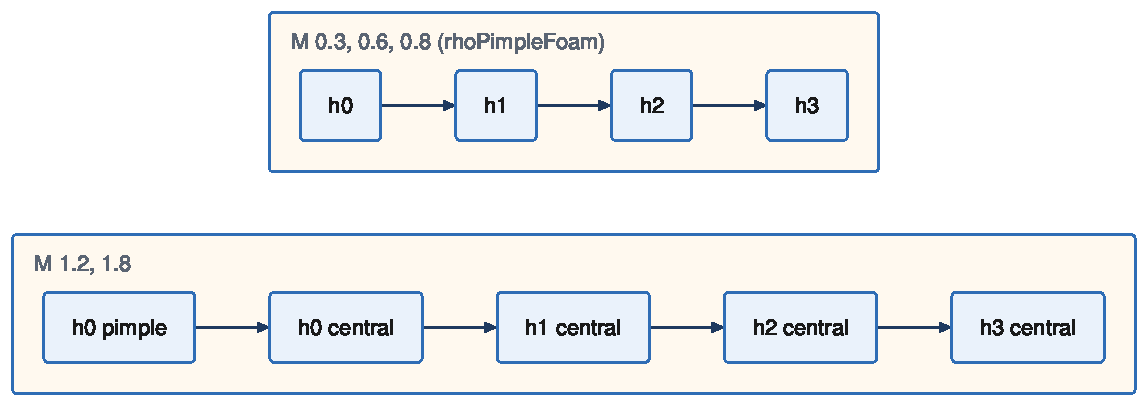
\includegraphics[width=0.95\linewidth]{figures/pdf/chains.pdf}
  \caption{Chains of runs. Left to right: from coarse to fine. Each arrow is an \texttt{--init}.}
  \label{fig:chains}
\end{figure}

A supersonic chain starts with a \cmd{rhoPimpleFoam} run on the coarsest mesh, because
\cmd{rhoCentralFoam} from a uniform free stream fails at the base
(\cref{sec:supersonic-start}).

\subsection{Mesh series for the convergence study}\label{sec:mesh-convergence-setup}

\begin{steps}
\item Change only \ent{maxCellSize}, with a constant ratio, and keep all levels. All
  cell sizes then change by the same ratio.
\item Use a ratio that gives a refinement ratio of more than 1.3 in the representative
  cell size, as the method of \citet{celik2008} needs. An octree mesh does not refine
  uniformly: calculate the real ratio of each pair from the number of cells,
  $r = (N_\text{fine}/N_\text{coarse})^{1/3}$, and use it in \cref{sec:gci}.
\item Keep $t_1$ equal on all meshes (\cref{sec:layers}).
\item Run the same flight conditions on all meshes.
\end{steps}

\section{Make the meshes}\label{sec:run-mesh}

\file{meshes.txt} has one mesh on each line: a name, then the options of
\file{Allmesh}. Lines that start with \texttt{\#} have no effect.

\begin{shell}
./runMesh.sh [meshes-file] [meshes-dir]      # default: meshes.txt, ~/meshes
\end{shell}

For each line: if the mesh exists with the same options, \file{runMesh.sh} keeps it; if
the options differ, it stops; if not, it runs \file{Allmesh}. It does not compare the
geometry: after a change of the STL file, remove the old meshes. To make one mesh only,
give a file with that line.

\section{Run the cases}\label{sec:run-sweep}

A sweep file has one case on each line: a name, then the options of \file{newCase.sh}
(\cref{tab:newcase}). A mesh or an \ent{--init} without \texttt{/} is a name in
\file{<meshes-dir>} or \file{<runs-dir>}. The run of an \ent{--init} must come earlier
in the file.

\begin{shell}
m08-a00-h1  --mesh h1 --solver pimple --alpha 0 --Minf 0.8 --pInf <Pa> --Tinf <K> --init m08-a00-h0
\end{shell}

\begin{shell}
./runCase.sh [--np <N>] [--socket <S>] <sweep-file> [runs-dir] [meshes-dir]
\end{shell}

The defaults are the physical cores of one socket, \file{~/runs} and \file{~/meshes}.
The sweep files do not contain the number of processes, so the same file works on any
computer. An option on a line of the file overrides the option of \file{runCase.sh}.

For each line, \file{runCase.sh} skips the case if its directory exists, stops if the
mesh does not exist, runs \file{newCase.sh}, and runs \file{Allrun}. A failed run does
not stop the sweep. Thus, after a stop, run \file{runCase.sh} again: it continues from
the first case that does not exist.

\paragraph{Processes and sockets.} One process for each physical core of one socket,
bound to its core (\cref{sec:binding}), is the default. On a computer with two sockets,
run \file{sweepSubsonic.txt} with \ent{--socket 0} and \file{sweepSupersonic.txt} with
\ent{--socket 1} at the same time. Each chain must stay in one file, because the files
run in parallel.

\subsection{Start a sweep}

\begin{steps}
\item Do the steps of \cref{sec:prepare-computer}.
\item Start the sweep so that it continues when the terminal closes:
\begin{shell}
nohup ./runCase.sh <sweep-file> > ~/log.<sweep> 2>&1 &
\end{shell}
\item On the first case, examine the binding (\cref{sec:binding}) and the measurement
  files (\cref{sec:measurement}).
\end{steps}

\subsection{Stop a sweep}

\begin{steps}
\item Stop \file{runCase.sh} by its process number (\cmd{kill <pid>}). No new case
  starts; the current solver continues.
\item To stop the solver also, stop its \cmd{mpirun} (or \cmd{prterun}) by its process
  number. \file{Allrun} then reconstructs the last time, writes the record and stops
  the measurement.
\end{steps}

\begin{caution}
\file{runCase.sh} reads the sweep file while it runs. Do not edit the file in place
until the sweep stops.
\end{caution}

\section{Flight conditions}\label{sec:flight-conditions}

The conditions of each Mach number come from the flight telemetry
(\cref{ch:flight}): the ambient pressure and temperature at the height where the vehicle
passed that Mach number in the coast phase, with the atmosphere of the day of the
flight. The standard atmosphere can differ by tens of kelvin from the real one, which
changes the Mach number at a given speed, the density and the Reynolds number.
\file{cdFlight.py} prints the conditions; write them into the sweep files.

\section{Rules}

\begin{itemize}
\item Do not put meshes or runs in the repository. Put the STL file, \file{meshDict},
  \file{meshes.txt} and the sweep files in it.
\item When a change to \file{meshDict} changes the mesh, commit it with the
  \cmd{checkMesh} summary of the new mesh.
\end{itemize}
